\documentclass[a4paper,12pt]{article}

\usepackage[utf8]{inputenc}
\usepackage{listings}
\usepackage{graphicx}
\usepackage[margin=1in]{geometry}
\usepackage{listings}
\usepackage{float}

%\setlength{\parskip}{\baselineskip}

%opening
\title{Computer Vision - Proposal}
\author{Argentina Ortega Sáinz \\
        Nicolás Alfonso Laverde}
\date{November 20, 2014}


\begin{document}
\pagenumbering{gobble}
\maketitle
\pagenumbering{arabic}
%---------------------------------------------------------------------------------------------%
\section*{Virtual Whiteboard.}

The idea is to develop a tracking system for a predefined marker that can be used to paint as if it was a virtual whiteboard. The system would have the capabilities to recognize different “virtual markers” (but one at a time), each one with a different color, and to detect the strokes or traces made with them. Detected strokes are then draw.
The aim behind it is to be able to project the drawings (traces of the marker) into a screen using of a video beam, and even to the point of saving them. This will allow the digitalization of notes made by the user of the system (marker carrier), such as a teacher, for later distribution and inspection.
%---------------------------------------------------------------------------------------------%
\subsection*{Objective}
Design a vision system able to recognize the strokes made with a predefined marker in a flat surface and to transform the strokes into drawings for later projection.
\begin{itemize}
\item Design, calibrate and synchronize an orthogonal array of two cameras in order to capture videos simultaneously of a scene from different perspectives.
\item Process two videos from different perspectives in order to detect strokes performed by a pre-defined marker.
\item Simulate a whiteboard by drawing the detected strokes and later projecting the draws into a screen for visualization.
\end{itemize}
%---------------------------------------------------------------------------------------------%
\subsection*{Motivation}
Obtaining the position of a certain object in real time has other applications, most interesting for us the computation of position of a robot. By using a simple example such as the virtual whiteboard to familiarize ourselves with the Computer Vision concepts, it could be possible in the future to extend this method to a much more complex application.
%---------------------------------------------------------------------------------------------%
\subsection*{Description}
We will use an orthogonal arrange of cameras. This will allow us to reconstruct the 3D coordinates of the marker using 2D synchronized images, following a similar approach as mentioned in \cite{laganiere}. The board plane contains the "x" and "y" coordinates, which are obtained by the re-projection of points from the two view to the board plane. The "z" component (depth) will make two modes distinguishable: the “writing mode” and a “moving mode” . A similar approach is mentioned in \cite{zabulis}, but using hand gestures instead of markers.

\begin{figure}[H]
    \begin{center}
    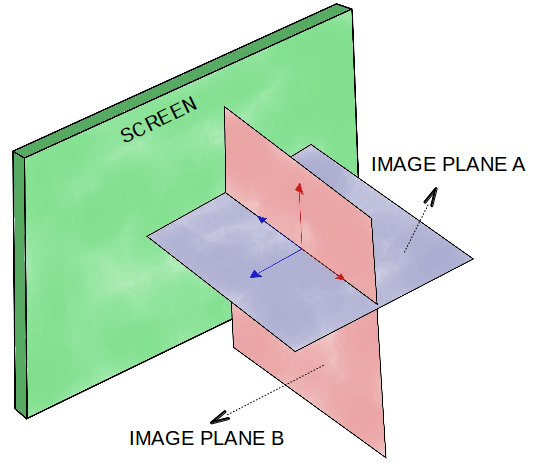
\includegraphics[width=8cm]{planesScheme.png}
    \caption{Planes Scheme.}
    The figure shows the three plains relevant to the system; the screen plane (in green) and  the two images planes (red and blue).
	\label{fig:planes}
    \end{center}
\end{figure}

The "writing mode" implies that the marker is close enough to the surface (screen) to enable the detection of the strokes, and therefore, drawing. The "moving mode" means that the marker can be moved, but the system will not detect the strokes of such movements, and therefore, no drawing is performed.

In other words, an "active drawing" volume is defined, which allow us to make the distinction between the modes. This active plane is parallel to the screen plane.

For the the system's output (drawing), we chose to back-project into the screen using a video-projector. Doing so, we can test the system at the same time; i.e. making the strokes and seeing the drawing correspondent to the movement of the marker. Projecting for the back allows us to avoid blocking the projected beam.

Detection of different colors in different markers will allow the user to paint on the screen. A possible approach is mentioned in \cite{fieguth}, \cite{mason} or \cite{McKenna}, to name a few.

%------------------------------------------------------------------------------------------------%
\subsection*{Set-Up}
The setup consists of two cameras arranged orthogonally; one camera is placed on the ceiling, over the board, and the other one is place in the side. Both cameras are to be mounted as close to the board as possible.

The selected cameras are two LiveCam from Microsoft, connected via USB. They have a frame rate of 30fps and a high resolution (up to 1920x1080). Additional, it offers an auto-focus feature from 0.1m to 10m.

\begin{figure}[H]
    \begin{center}
	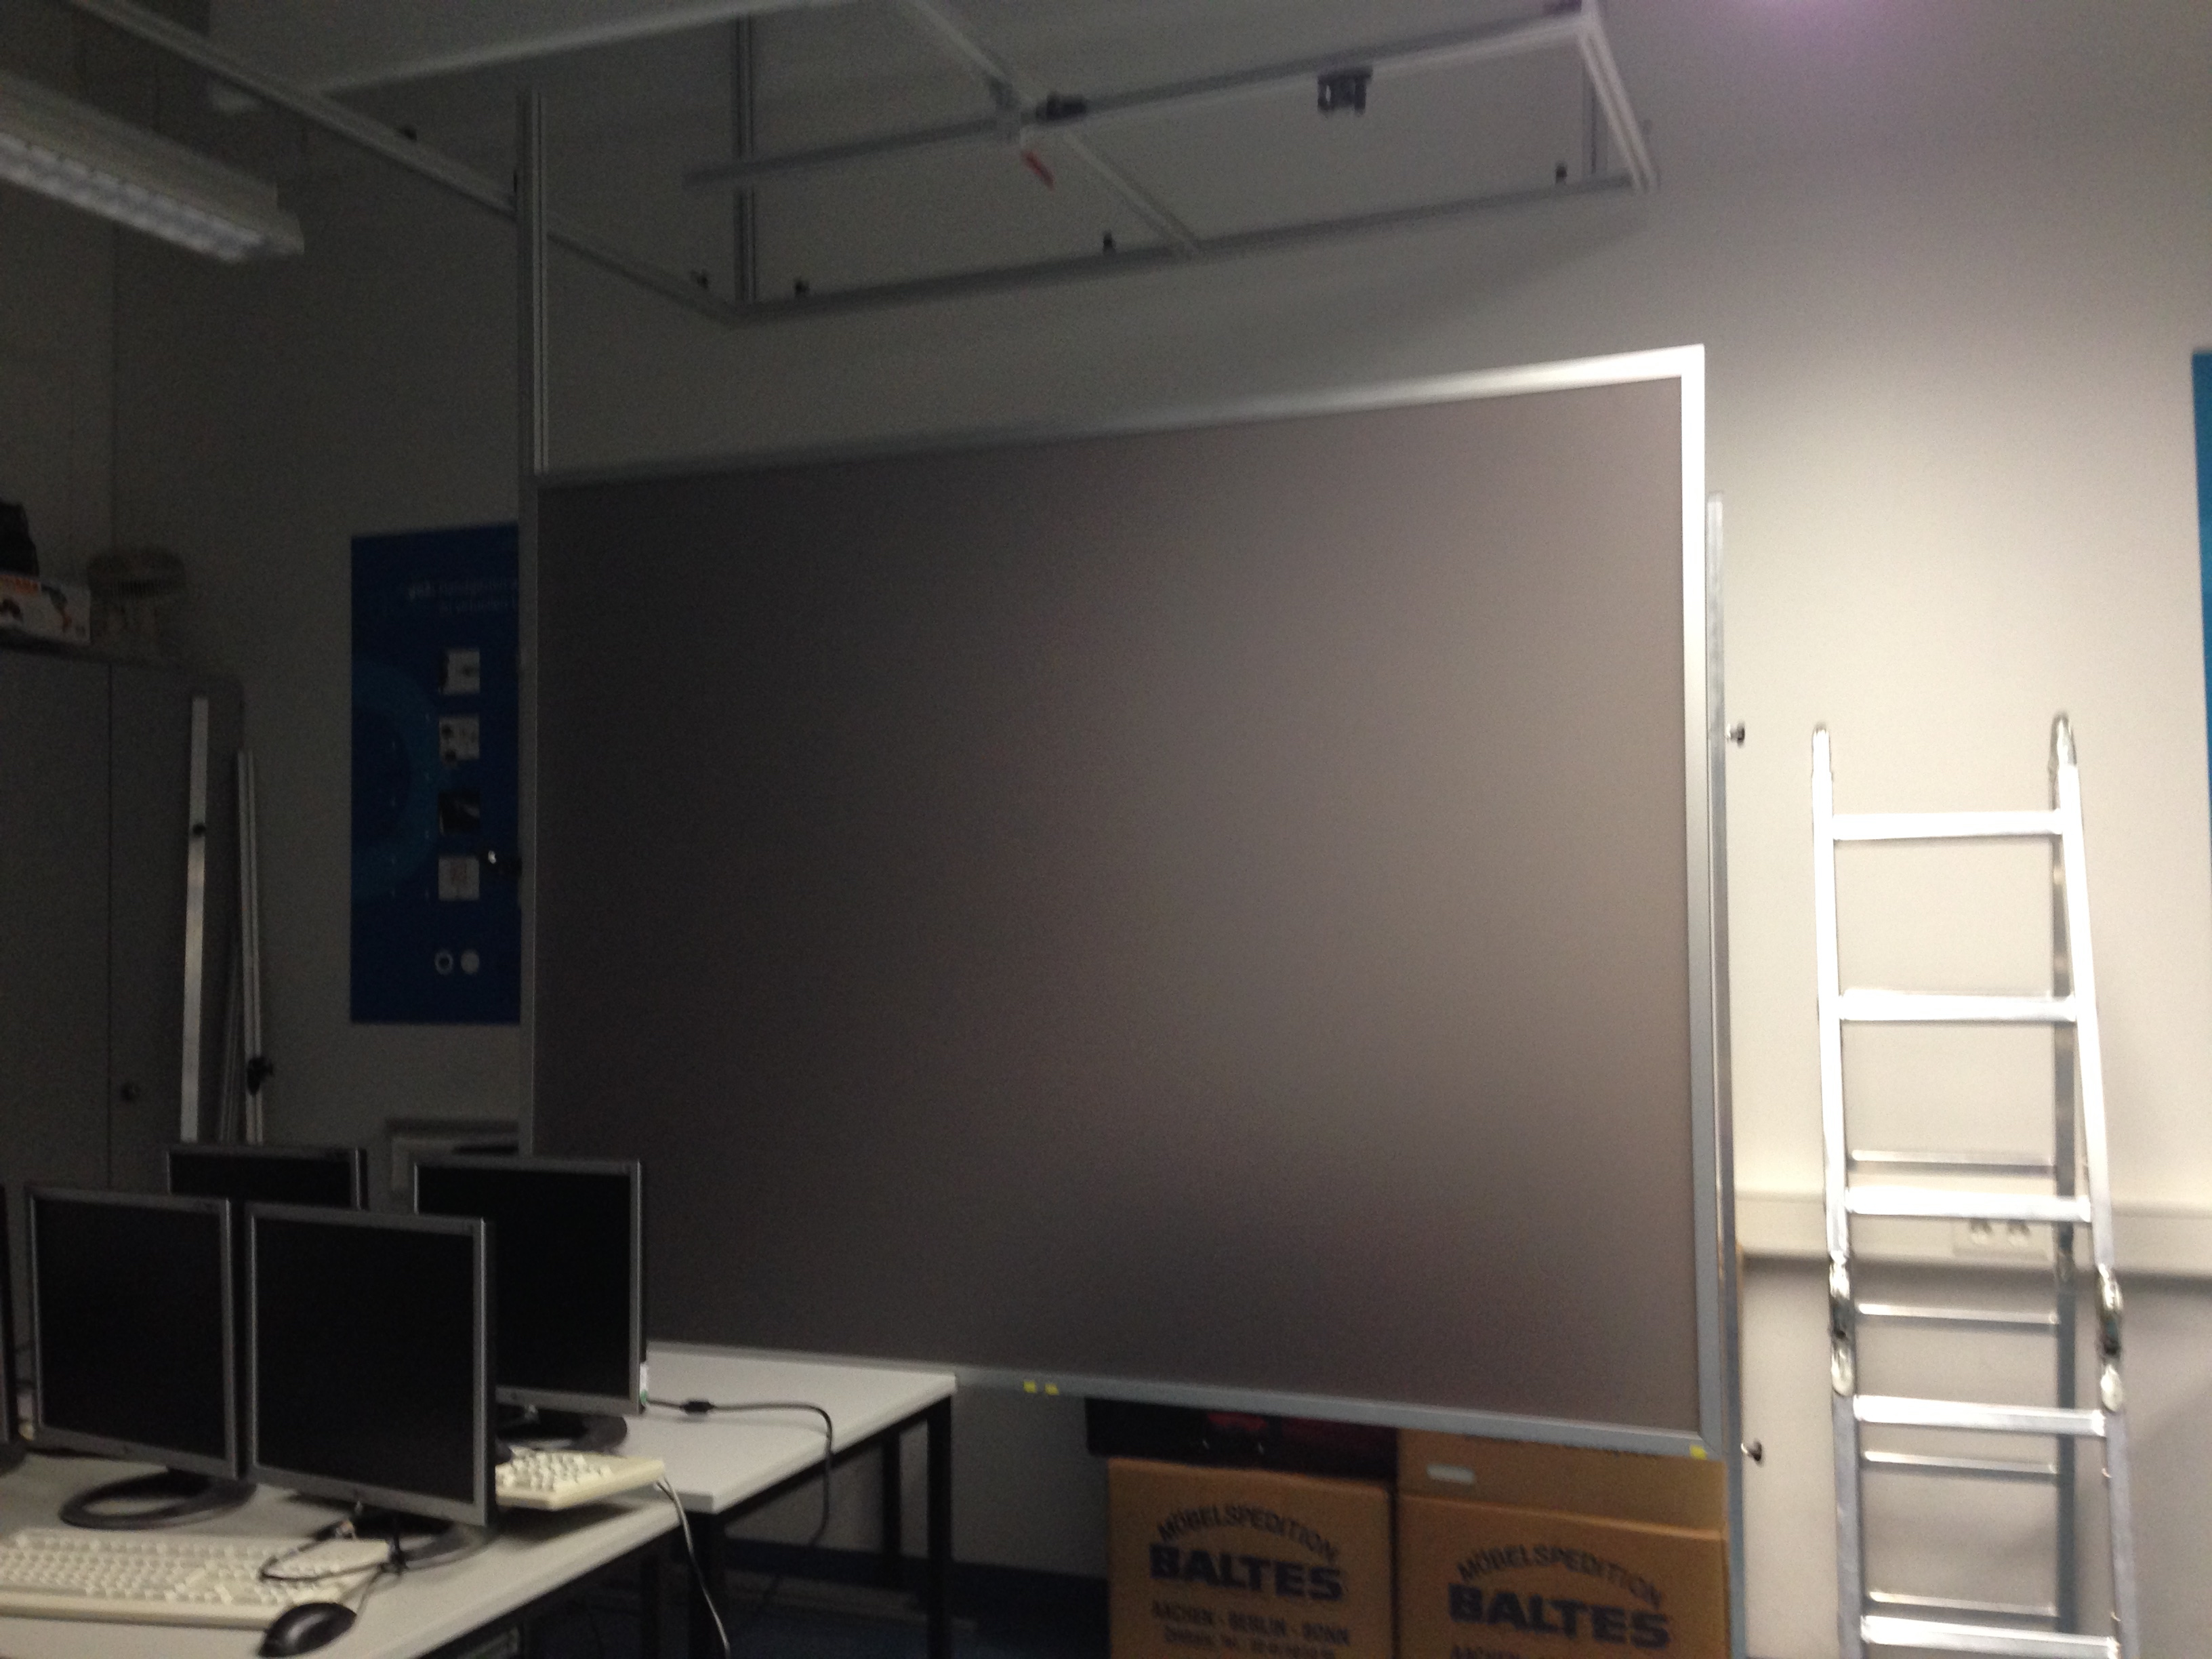
\includegraphics[width=12cm]{setup}
	\caption{Initial setup.}
    In the picture, the glass screen which allows us to back-project. The setup also illustrates the position of the cameras as well as the additional light source.
	\label{fig:setup}
    \end{center}
\end{figure}

A halogen lamp was added as a result of non-uniform lighting in the room (as seen in the picture).

\begin{figure}[H]
    \begin{center}
	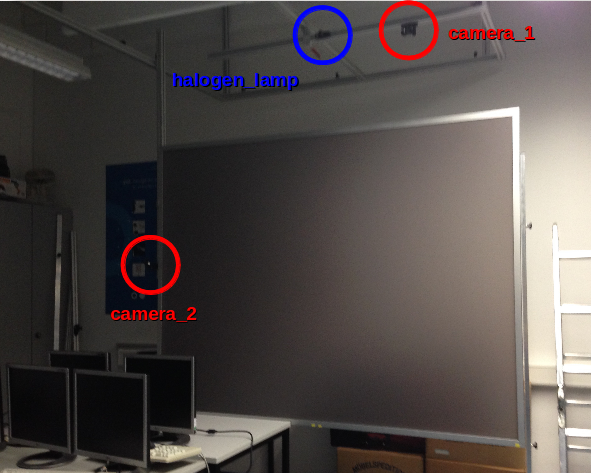
\includegraphics[width=12cm]{setupCams}
	\caption{Camera mounts and Light source positions.}
    The red circles indicate where the mounts for the cameras are. The blue circle indicates the position of the halogen lamp.
	\label{fig:setupcams}
    \end{center}
\end{figure}

\begin{figure}[H]
    \begin{center}
	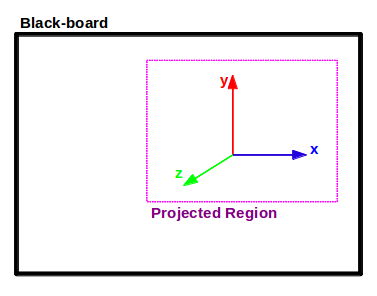
\includegraphics[width=8cm]{boardCoordinates}
	\caption{Board coordinate frame.}
    The purple dashed line corresponds to the effective area, where the video-beam will project the drawn strokes. This due to limitation in the distance between the video-beam and the physical screen
	\label{fig:board}
    \end{center}
\end{figure}

%---------------------------------------------------------------------------------------------%
\subsection*{Data}
As initialization a snapshot, one for each camera, is taken of the static background in order to be able to use them for segmentation later in the project. In addition, four snapshots are taken with the marker on each corner

Our data consists of snapshots of each perspective taken by each camera respectively. The resolution of the images is 1920 x 1080 and a predefined number of frames was recorded while the strokes were being drawn. 

These images are then processed by a PC generating the output, which consists of an image where the strokes are reprojected.

%Our data consists in two videos of a scene captured with two cameras, each one giving us a different perspective. For design purposes, we will take videos of approx. 5 min duration, in which some strokes will be recorded. Using this, we will develop the detection and drawing system.

%For the live demo, the system is supposed to work over on-line, meaning that the data for the cameras is streamed to a PC, where it is processed. The output of the system is then fed to a video-projector.

%---------------------------------------------------------------------------------------------%
%\subsection*{Assumptions}

%\begin{itemize}
%\item The cameras need to be calibrated every session in which video recording is intended, to reduce errors when computing the coordinates of the marker. Such calibration is needed because our physical board (glass screen) is mobile and it's possible that between sessions, the board has been moved by third parties.
%\item The image plane of camera A is rotated 90 degrees with respect to the image plane of camera B along the y-axis. For such assumption, the cameras have to be mounted in an specific arrange shown in the set-up section.
%\item The marker is sufficiently long in order to minimize occlusions. The color of the draw is chosen with the lid of the marker, so it has to be presented in the scene and in the tip of the marker.
%\item Given that our set up uses a glass screen which is very delicate, a special non-non-marking object will be provided to avoid scratch the screen.
%\end{itemize}

%---------------------------------------------------------------------------------------------%

\subsection*{Approach}
%Following a similar approach as the one mentioned in \cite{conci}, but adapted to our needs, we decided to divide the project in the following tasks:
The project was divided in the following sub-tasks:
\begin{itemize}
    \item Video capture. This stage consist in the recording of the video from the two cameras. This is in general terms our input data. For this stage we have taken into account:
    \begin{itemize}
        \item  Control of the environment. Lighting conditions, external sources of noise and occlusions were addressed during Set-up.
        \item Calibration of the cameras each time we want to record in a different work session. The calibration is needed given that the board (glass screen) can be moved from session to session. Autocalibration techniques consist of obtaining the intrinsic parameters of the camera based on principles of multiple view geometry, obtaining the fundamental matrix or using a Euclidean reconstruction. Two methods are available: Direct \cite{mendoncca} or stratification \cite{faugeras}. For more information see the references.
        \item Synchronization of the videos. This was done by syncing threads through the use of thread events. Each time the first thread is ready to take a snapshot it notifies the second one, and then both proceed to take a snapshot at approximately the same time.
    \end{itemize}
 \item Marker detection. This was accomplished by using a selected Region of Interest, which had been converted to HSV color space. Previously selected lower and upper boundaries help us isolate the marker from the background. A median blur is applied. We use Otsu's binarization threshold to segment the marker from the scene, which calculates the threshold based on the histogram of the region of interest. This process is repeated for each frame, where only the region of interest is used during calculation in order to reduce the amount of data processed.
   
    %This step correspond to the detection of our region of interest which we will track in the whole video, being this region the point of the marker. As we mention, we intent to process the videos frame by frame, and we will have to be able to detect the same region in each one of the frames to keep a record of the motion of the marker. The tracking of the position represent the stroke (movement) made. Techniques such as edge detection or optical flow could serve us by analyzing which pixels in the image remain the same (in intensity or brightness). This reduces the area of interest in the video and therefore reduces the amount of data needed to be processed (for example by color detection).   
    \item Color recognition. Once the marker was detected, the area with the marker was analyzed iby means of histograms. The color was detected in the RGB color space by using the RGB values found at the center of the circle that encloses the marker at the corner configuration sequence. 
    %This stage deals with the identification of the color shown in the video. We will have to detect the pertinent region where our lid will be (back or front the marker) for later extract the color. In this step we have to analyze which color space is more suitable for easy recognition, such as RGB, RGB normalized, HSV and YCrCb. Color detection is in general based on the search of pixels of the area of interest in a certain color space using a histogram. In our case we will detect first a smaller area of interest (the tip of the marker) and then detect the color. Depending on the lighting conditions we might use a different color space.
  
    \item Position reconstruction. Once we have the marker detected in each frame, the next step is to get the world coordinates back from the image coordinates. Assuming we have calibrated the cameras to obtain the intrinsic and extrinsic parameters, and we are able to reconstruct the matrix P of the cameras, we could then transform the image coordinates of the marker to the world coordinates. Exploiting the fact that our cameras share an axis, from which we will determined if the marker is close enough to the board to activate the drawing mode, we can extract the $x_{camera-i}$ and $y_{camera-j}$ coordinates of the marker, transform them to world coordinates and re-project them to the frame of the board. The output of this step is a vector with the world coordinates which describes a stroke in the world frame.
    \item Stroke draw. The stroke vector obtained from the position reconstruction is used to draw the stroke back into the screen, using a video-beam to project. For this step we need to draw the stoke with the color previously recognized.
\end{itemize}

%All the tasks, except the video capture stage, can be achieved independently up to some degree, making them more general. This will allow us to divided the workload between the two of us, work in each of the task alone, and finally integrate all the "pieces" together to build the overall system.


%Additionally, a intermediate step which we call "Pre-processing" could help us reduce dimentionality of the data. This mid-step includes filtering (for smoothing and noise reduction). We can study the possibility of transforming the whole video to gray values, process which will reduce the processing time by compacting the 3 color matrix into one using gray scale. Of course, for the color recognition, gray images won't work.

%---------------------------------------------------------------------------------------------%
\subsection*{Results}

All intermediate test will be done using the video recorded in the initial setup. 
\begin{itemize}
\item Video captured simultaneously from both cameras. 
\begin{figure}[H]
    \begin{center}
	%\includegraphics[width=8cm]{Video}
	\caption{Two snapshots taken simultaneously.}

	\label{fig:board}
    \end{center}
\end{figure}

\item Identification of at least 3 colors to be used on three different markers.
\begin{figure}[H]
    \begin{center}
	%\includegraphics[width=8cm]{MarkerDetection}
	\caption{Marker detection}
    Marker detected in both views. This is then used to detect the color of the stroke.
	\label{fig:board}
    \end{center}
\end{figure}
\item Set of $(x,y)$ coordinates of the movement "painted"
\item Algorithm that draws a line connecting a given set of points.
\end{itemize}
%---------------------------------------------------------------------------------------------%
%\subsection*{Risks}
%\begin{itemize}
%\item The computational power required by processing a synced input from two cameras could be a challenge as mentioned in \cite{martin}.
%\item The frame rate of the cameras has to be taking into account. A low frame rate means that fast moves will be hard to identify, while a high frame rate implies more frames to process.
%\item Illumination condition may inquire in difficulties when detecting the marker. Even when we have installed a halogen light source, we still could face some problems due to interference from other sources.
%\item Computational speed. We may suffer from a delay when drawing and projecting the detected strokes in the board due to the amount of processing we need in order produce the output. This could be seen if we make strokes in the board and the drawing is shown with some seconds (hopefully seconds) of delay.
%\item Depending on the frame rate of the cameras, we could suffer from systematic errors. This would imply that the accuracy of the drawing won't that the accuracy of the drawing won't be high, affected by the synchronization procedure mentioned before.
%\item The projected image has already a distortion due to the video-projector position. This could affect the measurement of the accuracy of the system.
%\end{itemize}

%---------------------------------------------------------------------------------------------%
%\subsection*{Evaluation Strategy}
%We propose to evaluate the system as following:
%\begin{itemize}
%\item Accuracy: using a projected grid,we choose some points as reference. Then, we will touch such points and compare the displacement of the projected points (output of the system) with the references (ground truth). One drawback of this evaluation strategy is the systematic errors introduced by the human user; e.g., a human can not guarantee 100\% accuracy when touching the grid points.
%\end{itemize}
%--------------------------------------------------------------------------------------------%

\nocite{*}

\bibliographystyle{unsrt}
\bibliography{Project}


%---------------------------------------------------------------------------------------------%
\end{document}